% Main Tài liệu dùng gói ex_test, phải đi kèm file ex_test.sty 
\documentclass[12pt,a4paper,twoside]{book}
\usepackage{fouriernc}
\usepackage{amsmath,amssymb,arcs,currfile}
\usepackage{tikz,tkz-tab,tkz-linknodes,tkz-euclide,tikz-3dplot,pgfplots}
\usepackage[top=1.5cm, bottom=1.5cm, left=1.5cm, right=1.5cm] {geometry}
\usepackage[dethi]{ex_test}
% \usepackage[loigiai]{ex_test}
% \usepackage[book]{ex_test}
% \usepackage[color]{ex_test}
% \usepackage[solcolor]{ex_test}
%\input{C:/texlive/Khai-bao-cho-file-main}
% \renewcommand{\baselinestretch}{1.2}
%%%%%%%%%%%%%%%%%\
\begin{document}
	\Opensolutionfile{ans}
	%-------------------------
	
\begin{tikzpicture}[>=stealth,line width=1pt,color=red]
\draw[->](-3,0)->(11,0);		%Vẽ trục số
\def\skipInterval{0.5cm}		%Khoảng cách đặt nhãn
\def\colorInterval{blue} 	%Màu tick, màu fill miền
\IntervalR{\big(}{2}{\big]}{5}
\end{tikzpicture}
\begin{center}
	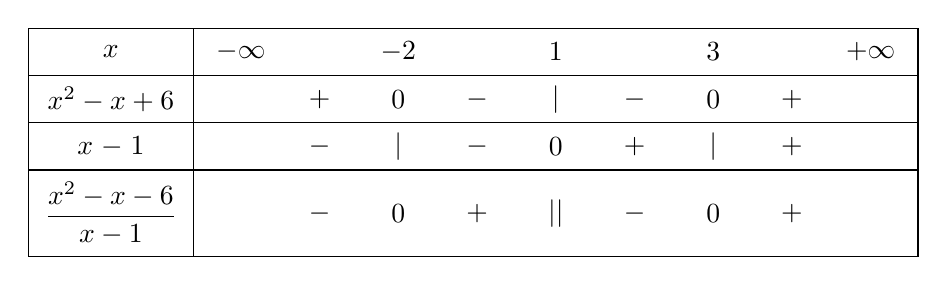
\begin{tikzpicture}
		\tkzTabInit[nocadre=false,lgt=2.1,espcl=2,deltacl=0.6]
		{$x$ /0.6,$x^2-x+6$ /0.6,$x-1$ /0.6,$\dfrac{x^2-x-6}{x-1}$ /1.1}
		{$-\infty$,$-2$,$1$,$3$,$+\infty$}
		\tkzTabLine{,+,$0$,-,|,-,$0$,+,}
		\tkzTabLine{,-,|,-,$0$,+,|,+,}
		\tkzTabLine{,-,$0$,+,||,-,$0$,+,}
	\end{tikzpicture}
\end{center}
\tikzset{double style/.append style={double distance=1.5pt}}
\begin{center}
	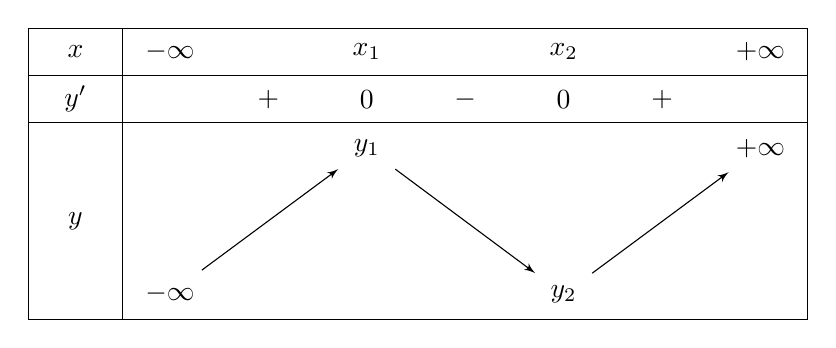
\begin{tikzpicture}
		\tkzTabInit[nocadre=false,lgt=1.2,espcl=2.5,deltacl=0.6]
		{$x$ /0.6, $y'$ /0.6, $y$ /2.5}
		{$-\infty$,$x_1$,$x_2$,$+\infty$}
		\tkzTabLine{,+,$0$,-,$0$,+,}
		\tkzTabVar{-/$-\infty$,+/$y_1$,-/$y_2$,+/$+\infty$}
	\end{tikzpicture}
\end{center}

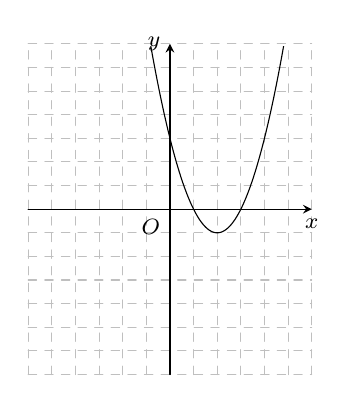
\begin{tikzpicture}[scale=0.3,>=stealth, font=\footnotesize, line join=round, line cap=round]
	\def\a{1} \def\b{-4} \def\c{3} % Hệ số
	\def\xmin{-6} \def\xmax{6}
	\def\ymin{-7} \def\ymax{7}
	
	\draw[color=gray!50,dashed] (\xmin,\ymin) grid (\xmax,\ymax);
	
	\draw[->] (\xmin,0)--(\xmax,0) node [below]{$x$};
	\draw[->] (0,\ymin)--(0,\ymax) node [left]{$y$};
	\node at (0,0) [below left]{$O$};
	\clip (\xmin+0.1,\ymin+0.1) rectangle (\xmax-0.5,\ymax-0.1);
	\draw[smooth,samples=300] plot(\x,{\a*(\x)^2+\b*(\x)+\c});
\end{tikzpicture}
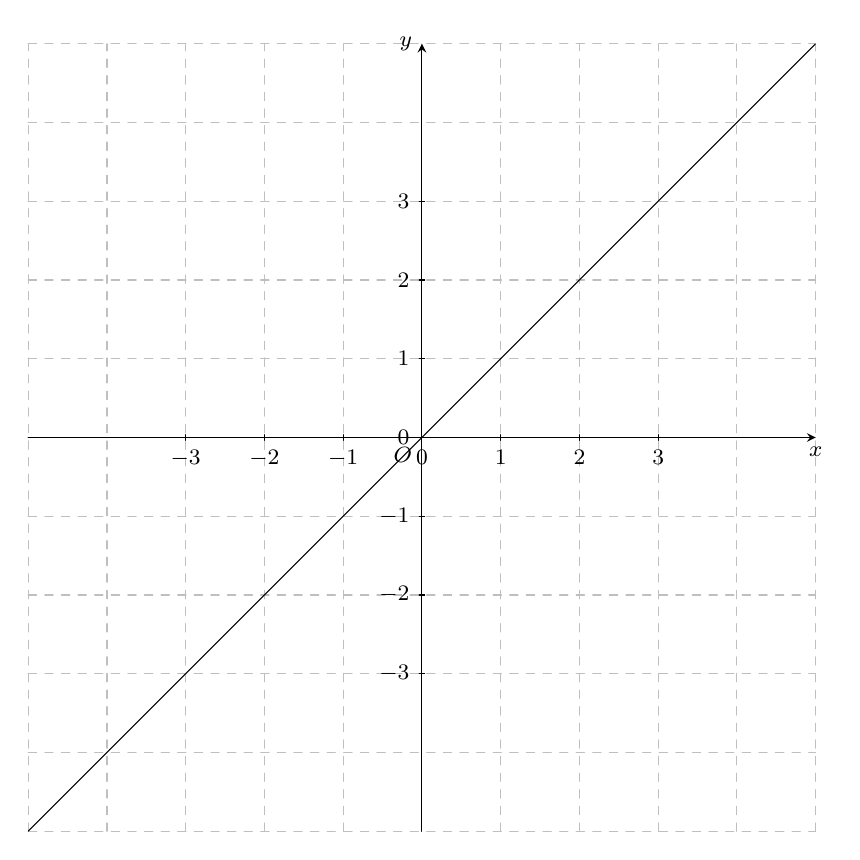
\begin{tikzpicture}[scale=1,>=stealth, font=\footnotesize, line join=round, line cap=round]
	\draw[color=gray!50,dashed] (-5,-5) grid (5,5);
	\draw[->] (-5,0)--(5,0) node [below]{$x$};
	\draw[->] (0,-5)--(0,5) node [left]{$y$};
	\node at (0,0) [below left]{$O$};
	\clip (-5,-5) rectangle (5,5);
	\draw[smooth,samples=300] plot(\x,{\x});
	\foreach \x in {-3,-2,...,3}
	\draw[thin] (\x,1pt)--(\x,-1pt) node [below] {$\x$};
	\foreach \y in {-3,-2,...,3}
	\draw[thin] (1pt,\y)--(-1pt,\y) node [left] {$\y$};
	
\end{tikzpicture}

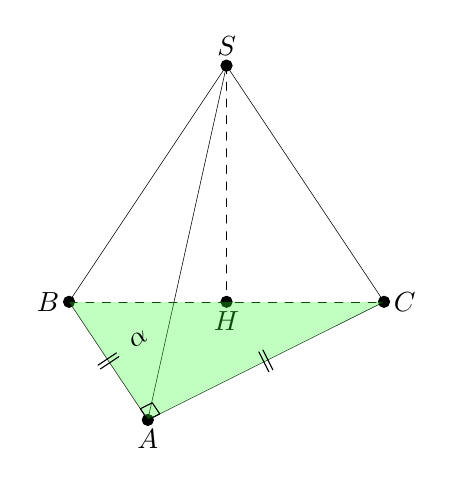
\begin{tikzpicture}[scale=1,>=stealth, font=\footnotesize, line join=round, line cap=round]
	\tkzDefPoints{0/0/B,1/-1.5/A,4/0/C}
	\coordinate (H) at ($(B)!0.5!(C)$);
	\coordinate (S) at ($(H)+(0,3)$);
	\tkzDrawPolygon(S,B,A,C)
	\tkzDrawSegments(S,A)
	\tkzDrawSegments[dashed](S,H)
	\tkzDrawSegments[dashed](B,C)
	\tkzDrawPoints[fill=black,size=4](A,B,C,S,H)
	\tkzLabelPoints[above](S)
	\tkzLabelPoints[below](H,A)
	\tkzLabelPoints[left](B)
	\tkzLabelPoints[right](C)
	\tkzFillPolygon[color=green!80, fill opacity=0.3](A,B,C)
	\tkzLabelAngles[pos=1,rotate=30](A,B,C){$\alpha$}
	\tkzMarkSegments[mark=||](A,B A,C)\tkzMarkRightAngles[size=0.17](B,A,C)
		
\end{tikzpicture}


	%-------------------------
	\Closesolutionfile{ans}
	
\end{document}